\section{Redes neurais na aprovação de empréstimos}\label{sec:rn}

Nesta parte do trabalho a base muda: em vez de moléculas, pedidos de empréstimo. A tarefa é prever se um pedido foi aprovado, e o modelo principal é uma rede neural do tipo perceptron de múltiplas camadas (MLP), comparada com os modelos das seções anteriores. Além da acurácia, registramos o tempo de treino de cada modelo.

\subsection{Dados e curadoria}

A base é o \emph{Loan-Approval-Prediction-Dataset}, publicado no Kaggle~\cite{kaggle:loan}: \rnLinhas{} pedidos, cada um com um identificador, 11 atributos e o rótulo (aprovado ou rejeitado). A Tabela~\ref{tab:rn_atributos} lista os atributos com os nomes usados neste trabalho. A página não informa a moeda; como o score é o do CIBIL, o birô de crédito da Índia, os valores devem estar em rúpias. Isso não afeta os modelos, que só comparam valores entre si.

\begin{table}[ht]
\centering
\caption{Atributos da base de empréstimos: nome no arquivo original, nome usado neste trabalho e faixa de valores. Valores em dinheiro em milhões, na moeda da base.}
\label{tab:rn_atributos}
\footnotesize
\begin{tabular}{lll}
\toprule
Coluna original & Nome neste trabalho & Valores \\
\midrule
\texttt{no\_of\_dependents} & dependentes & 0 a 5 \\
\texttt{education} & graduado & 1 = \emph{Graduate}, 0 = \emph{Not Graduate} \\
\texttt{self\_employed} & autônomo & 1 = \emph{Yes}, 0 = \emph{No} \\
\texttt{income\_annum} & renda anual & 0,2 a 9,9 \\
\texttt{loan\_amount} & valor do empréstimo & 0,3 a 39,5 \\
\texttt{loan\_term} & prazo (anos) & 2 a 20, de 2 em 2 \\
\texttt{cibil\_score} & score de crédito & 300 a 900 \\
\texttt{residential\_assets\_value} & patrimônio residencial & 0 a 29,1 \\
\texttt{commercial\_assets\_value} & patrimônio comercial & 0 a 19,4 \\
\texttt{luxury\_assets\_value} & bens de luxo & 0,3 a 39,2 \\
\texttt{bank\_asset\_value} & saldo bancário & 0 a 14,7 \\
\texttt{loan\_status} & aprovado (rótulo) & 1 = \emph{Approved}, 0 = \emph{Rejected} \\
\bottomrule
\end{tabular}
\end{table}

A curadoria foi curta, porque a base não tem valores ausentes nem linhas repetidas. O arquivo baixado é conferido pelo seu \emph{hash} SHA-256, para garantir que todos os experimentos partem do mesmo arquivo. Os nomes de colunas e os textos vinham com espaços no início, que foram removidos. \rnNegativos{} pedidos tinham patrimônio residencial de $-$100 mil, um valor impossível. Como a taxa de aprovação nessas linhas (57\%) é próxima da geral (\rnAprovados\%), o valor parece um erro de digitação, e não um sinal sobre o pedido; as linhas foram mantidas e o valor foi trocado por 0, que já aparece em outros 45 pedidos. Por fim, os três textos (escolaridade, autônomo e situação) viraram 0 e 1.

\subsection{Análise exploratória}\label{sec:rn_eda}

\rnAprovados\% dos pedidos foram aprovados, cerca de \rnRazaoClasses{} aprovado para cada rejeitado: a base é moderadamente desbalanceada, e a acurácia sozinha engana, porque responder sempre ``aprovado'' já acerta \rnAprovados\%. Esse é o piso desta parte. Um atributo domina os demais: o score de crédito tem correlação de \rnCorrScore{} com a aprovação, enquanto o prazo tem \rnCorrPrazo{} e os outros nove ficam perto de zero. Os valores em dinheiro são redundantes entre si: a renda anual tem correlação de \rnCorrRendaValor{} com o valor do empréstimo e de \rnCorrRendaLuxo{} com os bens de luxo (Figura~\ref{fig:rn_corr}).

\begin{figure}[ht]
\centering
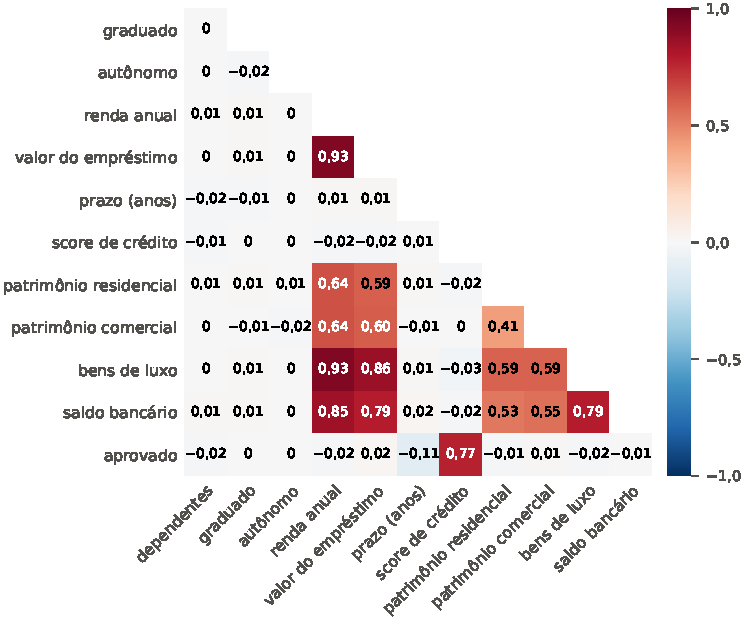
\includegraphics[width=.8\textwidth]{figures/rn_correlacao.pdf}
\caption{Correlação de Pearson entre os 11 atributos e a aprovação, na base inteira (\rnLinhas{} pedidos). Só o score de crédito se relaciona fortemente com a aprovação; os valores em dinheiro se correlacionam entre si e quase nada com o alvo.}
\label{fig:rn_corr}
\end{figure}

A Figura~\ref{fig:rn_score} mostra a forma dessa relação, e ela não é gradual: abaixo de 550 pontos, cerca de \rnAprovAbaixo\% dos pedidos são aprovados, em qualquer faixa; a partir de 550, \rnAprovAcima\%. A regra ``aprovar se o score for de pelo menos 550'' acerta \rnRegraBase\% da base. Os aprovados abaixo de 550 têm todos prazo de 2 ou 4 anos (\rnAprovPrazoDois\% e \rnAprovPrazoQuatro\% de aprovação nesses prazos); com prazos maiores, nenhum pedido abaixo de 550 foi aprovado. Os rótulos seguem, portanto, quase uma regra explícita: um degrau no score, com uma exceção para prazos curtos.

\begin{figure}[ht]
\centering
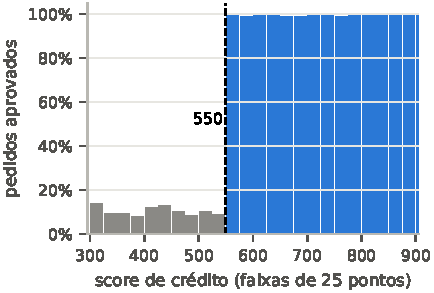
\includegraphics[width=.55\textwidth]{figures/rn_aprovacao_score.pdf}
\caption{Proporção de pedidos aprovados por faixa de 25 pontos de score de crédito. A linha tracejada marca 550.}
\label{fig:rn_score}
\end{figure}

A base parece sintética. O score e a renda se distribuem de forma quase uniforme: os quartis do score são 453, 600 e 748, contra 450, 600 e 750 de uma distribuição uniforme entre 300 e 900. Escolaridade e autônomo se dividem quase meio a meio. Com dados de crédito reais, seriam esperadas distribuições concentradas e uma relação mais gradual entre o score e a aprovação. Isso limita o alcance das conclusões (Seção~\ref{sec:limitacoes}).

\subsection{Metodologia}\label{sec:rn_metodo}

\textbf{Protocolo.} Os dados são divididos em treino (80\%, \rnTreino{} pedidos) e teste (20\%, \rnTeste), mantendo a proporção de aprovados, e o procedimento é repetido com 10 seeds (0 a 9), que mudam a divisão, as partes da validação cruzada e a semente dos modelos. Não há gêmeas como na base de moléculas, então a divisão é estratificada simples. Quando um modelo tem hiperparâmetros a escolher, uma busca em grade com validação cruzada estratificada de 5 partes, feita só dentro do treino, escolhe a combinação de maior acurácia. No teste, reportam-se acurácia, F1 macro, a área sob a curva ROC (AUC) e, para a rede e a árvore, a matriz de confusão. O desbalanceamento é tratado pela divisão e pela validação estratificadas e por métricas que não favorecem a classe maior: o F1 macro, média simples do F1 das duas classes, a AUC, que não depende da proporção entre elas, e a matriz de confusão, que mostra o erro em cada uma. Não usamos reamostragem nem pesos por classe, porque a classe menor tem \rnRejeitadosBase{} pedidos e os modelos acertam bem as duas classes. A AUC usa a probabilidade prevista, e não a classe: é a chance de um pedido aprovado, sorteado ao acaso, receber probabilidade maior que um rejeitado. Ela mede, portanto, se o modelo ordena bem os pedidos, independentemente do corte em 50\%.

\textbf{Modelos de referência.} Cinco modelos servem de régua: a classe majoritária; a \emph{regra de um corte}, uma árvore de profundidade 1 que escolhe sozinha, no treino, o melhor atributo e o melhor limiar (escolheu o score e 549,5 nas 10 seeds); a regressão logística com padronização, que equivale a uma rede de um único neurônio; a árvore de decisão com busca em grade (critério, profundidade máxima e mínimo por folha, \rnCombinacoesArv{} combinações); e a Random Forest com 300 árvores.

\textbf{A rede neural.} A rede é um MLP do scikit-learn~\cite{pedregosa:11}: camadas ocultas com ativação ReLU~\cite{nair:10}, um neurônio de saída com sigmoide, que dá a probabilidade de aprovação, perda de entropia cruzada e otimizador Adam~\cite{kingma:15}. Antes da rede, cada atributo é padronizado (subtrai-se a média e divide-se pelo desvio padrão do treino, nunca do teste). O treino usa parada antecipada~\cite{prechelt:98}: 10\% do treino ficam de fora como validação, e o treino para quando a acurácia nessa validação passa um número fixo de épocas, a \emph{paciência}, sem melhorar. Usamos paciência de 30 épocas em vez das 10 do padrão do scikit-learn, pelo motivo mostrado na Seção~\ref{sec:rn_resultados}. A busca em grade cobre a arquitetura (8, 16, 32 ou 64 neurônios numa camada; 32 e 16 ou 64 e 32 em duas), a regularização L2 ($\alpha$ de $10^{-4}$ ou $10^{-2}$) e a taxa de aprendizado ($10^{-3}$ ou $10^{-2}$), \rnCombinacoes{} combinações.

\textbf{Tempo de execução.} Para comparar algoritmos, e não o número de núcleos que cada um usa, tudo roda num único núcleo (\texttt{n\_jobs=1} e as bibliotecas de álgebra linear limitadas a uma \emph{thread}). Antes da primeira medição, uma rodada de aquecimento é feita e descartada. Nos modelos com busca em grade, o tempo da busca é medido à parte, e o modelo final é treinado de novo com os hiperparâmetros escolhidos para medir só o treino. O resumo usa a mediana das 10 seeds. A máquina é um AMD Ryzen 5 9600X (6 núcleos) com 31 GB de memória, Windows 11, Python 3.14 e scikit-learn 1.9.1, sem outras tarefas pesadas durante a execução.

\subsection{Resultados}\label{sec:rn_resultados}

\textbf{Padronização.} A mesma rede, com 16 neurônios numa camada, acerta \rnSemPadAcc~$\pm$~\rnSemPadSd\% sem padronização, abaixo do piso de \rnAprovados\%, com AUC de \rnSemPadAuc\%, o mesmo que sortear. Com padronização, acerta \rnComPadAcc~$\pm$~\rnComPadSd\%. Sem ela, a renda e os patrimônios, na casa dos milhões, dominam a soma ponderada de cada neurônio, e o passo do otimizador, do mesmo tamanho para todos os pesos, não serve ao mesmo tempo para atributos de 0 a 5 e de 0 a 40 milhões~\cite{lecun:98}. A árvore não sofre com isso, porque compara cada atributo apenas com um limiar.

\textbf{Neurônios.} A Figura~\ref{fig:rn_neuronios} mostra a acurácia de validação cruzada (seed 42) por número de neurônios. Com 1 neurônio por camada, a rede fica perto da regressão logística (\rnNeurUm\% com uma camada). Com 2 a 8 neurônios, já passa de 97\%, e o melhor ponto, duas camadas de 8, chega a \rnNeurOitoDuas\%, perto da árvore. Mais neurônios não ajudam: com 64 numa camada, a acurácia cai para \rnNeurSessentaQuatro\%. A curva é irregular porque cada ponto é uma única rede, e o resultado depende dos pesos iniciais sorteados.

\begin{figure}[ht]
\centering
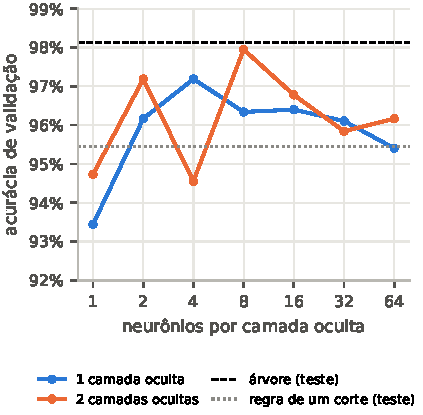
\includegraphics[width=.5\textwidth]{figures/rn_neuronios.pdf}
\caption{Acurácia de validação cruzada (5 partes, seed 42) por número de neurônios em cada camada oculta, com taxa de aprendizado de $10^{-2}$ e sem parada antecipada. As linhas horizontais são a acurácia de teste da árvore e da regra de um corte (média de 10 seeds).}
\label{fig:rn_neuronios}
\end{figure}

\textbf{Épocas e paciência.} Cada época é uma passada completa pelo treino. A Figura~\ref{fig:rn_epocas} acompanha uma rede de 32 neurônios por 400 épocas, sem parada antecipada. A perda de treino continua caindo, enquanto a de validação se estabiliza: a partir daí, a rede passa a ajustar detalhes do treino que não se repetem na validação (Figura~\ref{fig:rn_epocas}a). Com taxa de aprendizado de $10^{-3}$, a rede aprende devagar, e a acurácia de validação passa longos trechos sem melhorar. Com paciência 10, o treino pararia na época \rnParadaLentaDez{}, com \rnParadaAccLentaDez\% de validação, quando a mesma rede chegaria a \rnMelhorLenta\%; com paciência 30, para na época \rnParadaLentaTrinta{}, com \rnParadaAccLentaTrinta\% (Figura~\ref{fig:rn_epocas}b). Com taxa de $10^{-2}$, chega a 97\% em menos de 100 épocas. A busca em grade confirmou o quadro: escolheu a taxa de $10^{-2}$ em \rnSeedsTaxa{} das 10 seeds e duas camadas ocultas em \rnSeedsDuas{} (32 e 16 neurônios em \rnSeedsTrintaDezesseis), e a rede final treinou de \rnEpocasMin{} a \rnEpocasMax{} épocas.

\begin{figure}[ht]
\centering
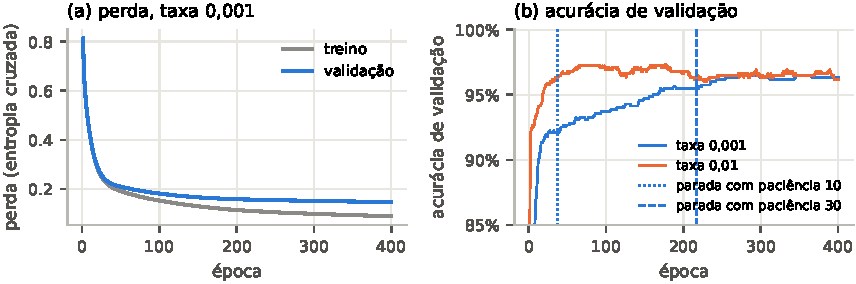
\includegraphics[width=\textwidth]{figures/rn_epocas.pdf}
\caption{Uma rede de 32 neurônios treinada por 400 épocas (seed 42; 80\% do treino para ajustar e 20\% para validar). (a) Perda no treino e na validação, com taxa de aprendizado de $10^{-3}$. (b) Acurácia de validação com as duas taxas; as linhas verticais marcam onde a parada antecipada interromperia a rede de taxa $10^{-3}$ com paciência de 10 e de 30 épocas.}
\label{fig:rn_epocas}
\end{figure}

\textbf{Comparação com os modelos de referência.} A Tabela~\ref{tab:rn_modelos} reúne os seis modelos. A rede acerta \rnAccRede~$\pm$~\rnSdRede\%. Comparando seed a seed, ela supera a regressão logística em todas as 10 seeds (\rnDifRedeLog{} pontos), o que mostra o ganho das camadas ocultas sobre um neurônio só, e supera a regra de um corte em \rnSeedsRedeRegra{} das 10 (\rnDifRedeRegra{} ponto, menos que o desvio entre seeds). Perde para a árvore de decisão em todas as seeds (\rnDifRedeArv{} ponto) e para a Random Forest em 9 (\rnDifRedeRF{} ponto). Também é o modelo menos estável: o desvio de \rnSdRede{} ponto é quase três vezes o da árvore. A AUC conta outra parte da história. A da rede (\rnAucRede\%) é maior que a da árvore (\rnAucArv\%), assim como a da regressão logística (\rnAucLog\%) é maior que a da regra de um corte (\rnAucRegra\%), que acerta mais: os modelos de saída suave ordenam bem os pedidos, e o que erram é o corte em 50\%. Árvore e Random Forest empatam (\rnDifRFArv{} ponto, a floresta melhor em \rnSeedsRFArv{} das 10 seeds).

\begin{table}[ht]
\centering
\caption{Os seis modelos na base de empréstimos (média $\pm$ desvio em 10 seeds; erros em \rnTeste{} pedidos de teste). Tempos: mediana das 10 seeds, num único núcleo. Treino: o do modelo final; busca: a busca em grade com validação cruzada de 5 partes; previsão: os \rnTeste{} pedidos de teste.}
\label{tab:rn_modelos}
\footnotesize
\setlength{\tabcolsep}{4pt}
\begin{tabular}{lccccccc}
\toprule
Modelo & Acurácia (\%) & \shortstack{F1 macro\\(\%)} & AUC (\%) & Erros &\shortstack{Treino\\(ms)} & \shortstack{Busca\\(s)} & \shortstack{Previsão\\(ms)} \\
\midrule
Classe majoritária & 62,2 $\pm$ 0,0 & 38,3 & 50,0 & 323,0 & 0,2 & -- & 0,03 \\
Regra de um corte & 95,5 $\pm$ 0,6 & 95,3 & 96,2 & 38,8 & 1,9 & -- & 0,3 \\
Regressão logística & 91,9 $\pm$ 1,1 & 91,3 & 97,0 & 69,5 & 3,5 & -- & 0,5 \\
Árvore de decisão & 98,1 $\pm$ 0,4 & 98,0 & 98,7 & 16,0 & 3,7 & 0,65 & 0,3 \\
Random Forest & 98,3 $\pm$ 0,4 & 98,2 & 99,8 & 14,5 & 490 & -- & 15,3 \\
Rede neural (MLP) & 96,4 $\pm$ 1,1 & 96,1 & 99,3 & 30,9 & 183 & 23,5 & 0,6 \\
\bottomrule
\end{tabular}

\end{table}

\textbf{Tempo.} Treinar a rede final leva \rnTreinoRedeMs{} ms, cerca de \rnRazaoTreino{} vezes os \rnTreinoArvMs{} ms da árvore, e menos da metade dos \rnTreinoRFMs{} ms da Random Forest. O maior custo da rede está na escolha dos hiperparâmetros: a busca leva \rnBuscaRede{} s por seed, contra \rnBuscaArv{} s da árvore (\rnRazaoBusca{} vezes mais), porque cada uma das \rnCombinacoes{} combinações treina 5 redes por dezenas de épocas. Prever é rápido para quase todos: \rnPrevRedeMs{} ms para a rede e menos de 1 ms para a árvore, contra \rnPrevRFMs{} ms da Random Forest, que consulta 300 árvores.

\textbf{Onde a rede erra.} Na seed 42, a rede comete \rnErrosRedeSeed{} erros no teste, e a árvore, \rnErrosArvSeed. Os erros da rede se concentram logo acima do degrau: entre 550 e 599 pontos há \rnPedidosFaixa{} pedidos de teste, e a rede erra \rnErrosRedeFaixa{}, contra \rnErrosArvFaixa{} da árvore. A árvore, por sua vez, erra sobretudo na exceção dos prazos curtos (score abaixo de 550 e prazo de até 4 anos, \rnExcecao{} pedidos): \rnErrosArvExc{} dos seus \rnErrosArvSeed{} erros, contra \rnErrosRedeExc{} da rede. A Figura~\ref{fig:rn_rampa} mostra a causa. A árvore representa o degrau com uma pergunta e dá probabilidades de 0 ou 100\% em quase todos os pedidos. A rede desenha uma rampa: entre 500 e 599 pontos, \rnInterRede\% das suas probabilidades ficam entre 10\% e 90\%, contra \rnInterArv\% na árvore, e é nessa rampa que estão os seus erros. Redes neurais tendem a aprender funções suaves, e uma relação em degrau é justamente o caso em que modelos de árvore costumam levar vantagem em dados tabulares~\cite{grinsztajn:22}.

\begin{figure}[ht]
\centering
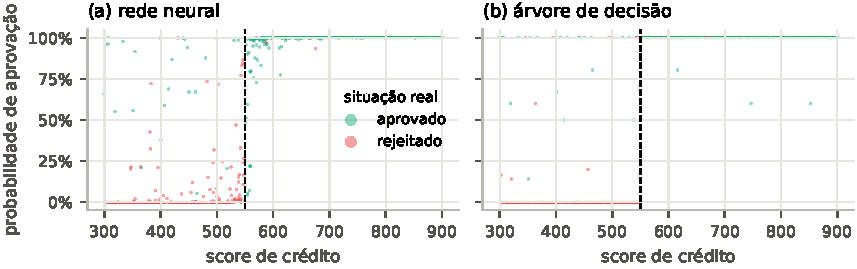
\includegraphics[width=\textwidth]{figures/rn_rampa_degrau.pdf}
\caption{Probabilidade de aprovação prevista para cada pedido de teste, por score de crédito (seed 42), colorida pela situação real. (a) Rede neural. (b) Árvore de decisão. A linha tracejada marca 550.}
\label{fig:rn_rampa}
\end{figure}

\textbf{Tipos de erro.} Com a aprovação como classe positiva, um falso positivo é aprovar um pedido que foi rejeitado, o erro que expõe o banco a calote, e um falso negativo é recusar um pedido que foi aprovado, o que custa um bom cliente. Na seed 42 (Figura~\ref{fig:rn_confusao}), a rede tem \rnFPRedeSeed{} falsos positivos e \rnFNRedeSeed{} falsos negativos; a árvore, \rnFPArvSeed{} e \rnFNArvSeed. Quase toda a diferença está nos falsos negativos, a maioria deles entre 550 e 599 pontos, na rampa da rede. Na média das 10 seeds, porém, a rede erra mais dos dois lados: \rnFPRedeMed{} falsos positivos e \rnFNRedeMed{} falsos negativos por seed, contra \rnFPArvMed{} e \rnFNArvMed{} da árvore. Em proporção, a rede aprova \rnTaxaFPRede\% dos \rnTesteRej{} pedidos rejeitados do teste e recusa \rnTaxaFNRede\% dos \rnTesteAprov{} aprovados (árvore: \rnTaxaFPArv\% e \rnTaxaFNArv\%). Os dois modelos erram mais aprovando do que recusando: só em \rnSeedsFNRede{} das 10 seeds a rede tem mais falsos negativos que falsos positivos, e a árvore também em \rnSeedsFNArv. Se um calote custar mais que um cliente perdido, o corte de 50\% poderia ser elevado, escolhido na validação; não o fizemos, para manter o mesmo critério em todos os modelos.

\begin{figure}[ht]
\centering
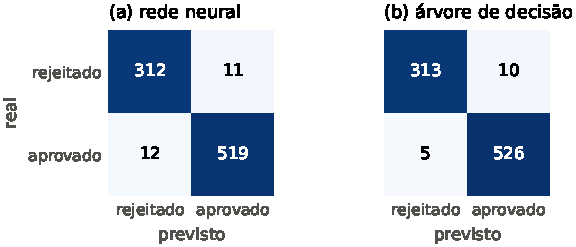
\includegraphics[width=.62\textwidth]{figures/rn_confusao.pdf}
\caption{Matriz de confusão no teste (seed 42, \rnTeste{} pedidos). (a) Rede neural. (b) Árvore de decisão. Cor pela proporção da classe real; número em contagem.}
\label{fig:rn_confusao}
\end{figure}
